\documentclass[12pt]{article}
\usepackage[utf8]{inputenc}
\usepackage[margin=1in]{geometry}
\usepackage{amsmath}
\usepackage{graphicx}
\usepackage{enumerate}
\graphicspath{ {./images/} }

\author{Neelu Saraswatibhatla (srns2)}
\title{Operating Systems Supervision 2}
\date{\vspace{-5ex}}

\begin{document}

\maketitle

\section{Example Sheet}

\subsection*{2.2}

\begin{enumerate}[(a)]
    \item This is true, as preemptive schedulers need hardware support in the form of a timer that can raise an interrupt and change the program counter to restore control to the OS after a given amount of time.
    \item This can be true, depending on how much memory the processes in progress use and how big the TLB is. If the TLB has enough space to store the contexts of all processes in progress, then simple flip-flops can be used to switch context by simply setting the program counter to the correct area of the TLB, but if the TLB is not large enough then the context must be stored in main memory, or even onto disk if really necessary.
    \item This is true, as the block device can just return data as it is being read. For example, a disk drive is a block device, but it can be used for non-blocking IO by passing data as it is read.
    \item This is false, as it means that longer jobs are not even guaranteed to be run, and even if they are they will have to wait a lot longer than they would in, for example, round robin. Furthermore, more time would be spent on context switching on average in SJF than in an algorithm like FCFS (which is also not an optimal algorithm but is better in this respect).
    \item This is false, as all jobs will get their quanta and one particularly slow job won't stop others from being run.
    \item This is not necessarily true. Even though external fragmentation doesn't exist in paged virtual memory, internal fragmentation does so just as much space may be wasted.
    \item This is false. It does not make the actual devices go faster, but frees up the OS from having to deal with as many interrupts, allowing the CPU to run processes faster.
    \item This is false, as system calls are required for everything from creating processes to accessing IO devices.
    \item This is true, as in order to have a hard link, the two file names must point to the same i-node, but i-nodes are filesystem-specific.
    \item This is true, if stdout or stderr is set to be the buffer cache.
\end{enumerate}


\subsection*{2.5}



\subsection*{2.6}

\begin{enumerate}[(a)]
    \item Internal fragmentation occurs in page tables, where there is empty space within a page but no empty space between pages. External fragmentation occurs in segmentation when there is empty space between segments. Internal fragmentation can be addressed by changing the page size, and external fragmentation can be addressed by compaction.
    \item A page table contains the address of the required page in memory. With a TLB, when a page table entry is requested, if it is in the TLB it is returned, and if not it is retrieved from main memory, and put in the TLB.
    \item In a single level page table, the base register points to a page table, and the virtual memory address contains the location of the page table entry within the page table, and the offset within the page. In a double level page table, the base register contains the first page table, but each entry in this page table points to another page table. Each entry in each of these second page tables points to a page. In this case, the virtual memory address contains the locations of the relevant entries in each of the two required page tables and the offset on the page. This concept of multilevel page tables can be extended to more than two page 2 levels if necessary. The reason for this is that most devices have huge address spaces which lead to very large page tables and we don't want to keep an entire page table in memory, so we split page tables into smaller ones in this way.\\
    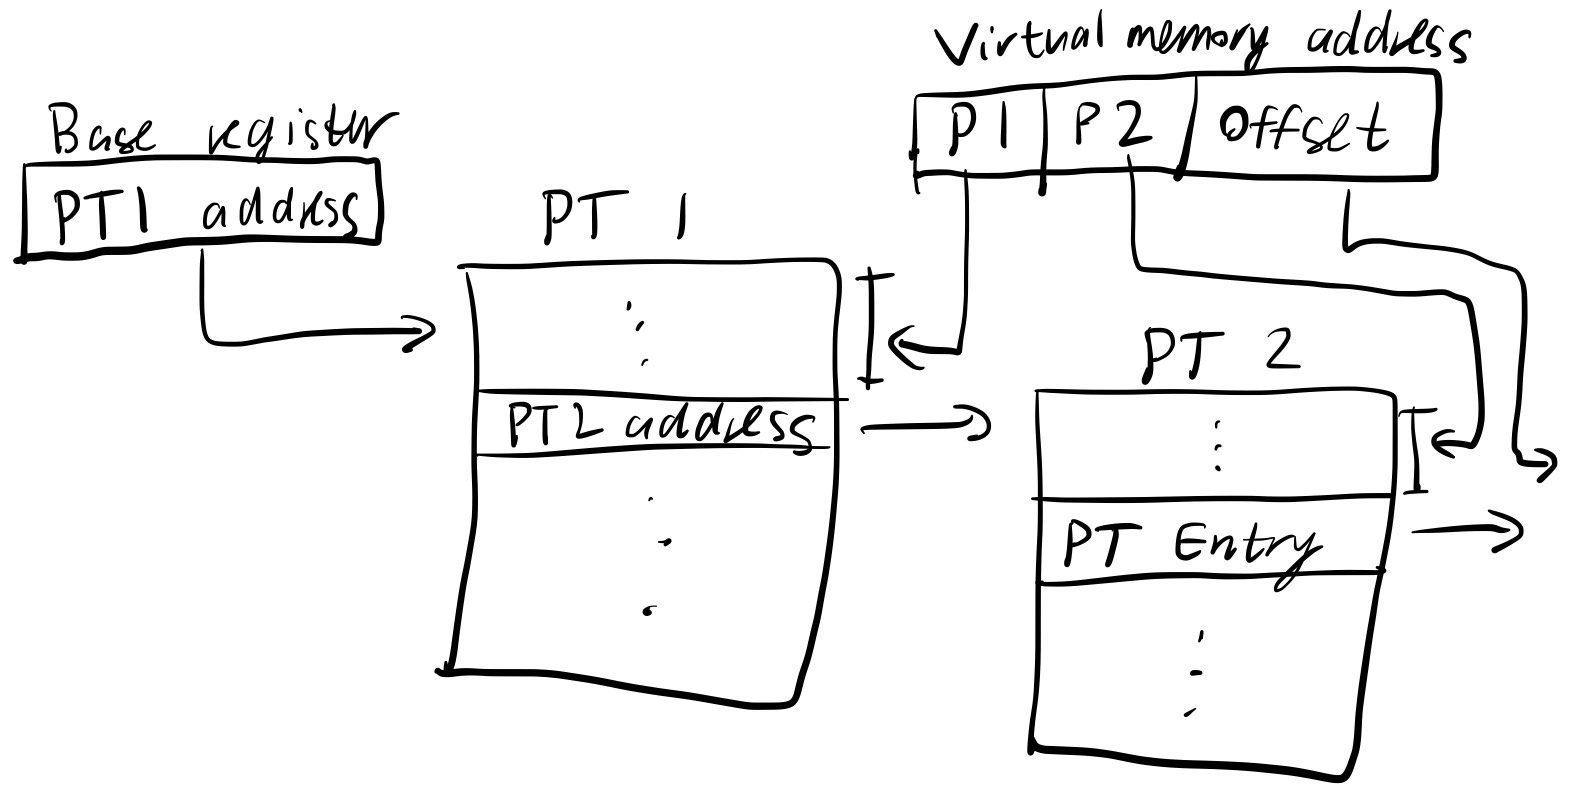
\includegraphics[scale=0.25]{2.6c.jpg}
\end{enumerate}

\subsection*{3.1}
\begin{enumerate}[(a)]
    \item It can directly access the IO devices.
    \item It raises an interrupt to the kernel, which accesses the IO device and does the required operation, and returns data and control to the process when appropriate.
\end{enumerate}

\subsection*{3.3}
With blocking IO, the process is suspended until the blocked IO returns. In the case of a keyboard, when the process blocks, the keyboard IO is read by the OS and once it has been read the OS may return control to the process.

With non-blocking IO, the device returns as much data as is available to the process instantly. In the case of a keyboard, if, for example, a key is being pressed at the moment the process requests IO, it is returned.

With asynchronous IO, the process runs while waiting for IO. In the case of a keyboard, the process may request input and then continue to do other tasks, and come back to process the keyboard input when it becomes available.

\subsection*{3.4}

\begin{enumerate}[(a)]
    \item The directory service maps names to file identifier, and handles access and existence control.
    \item In a directory hierarchy, directories have parents and children, and the children can be other directories or files. For example, in Unix the hierarchy may look something like this:\\
    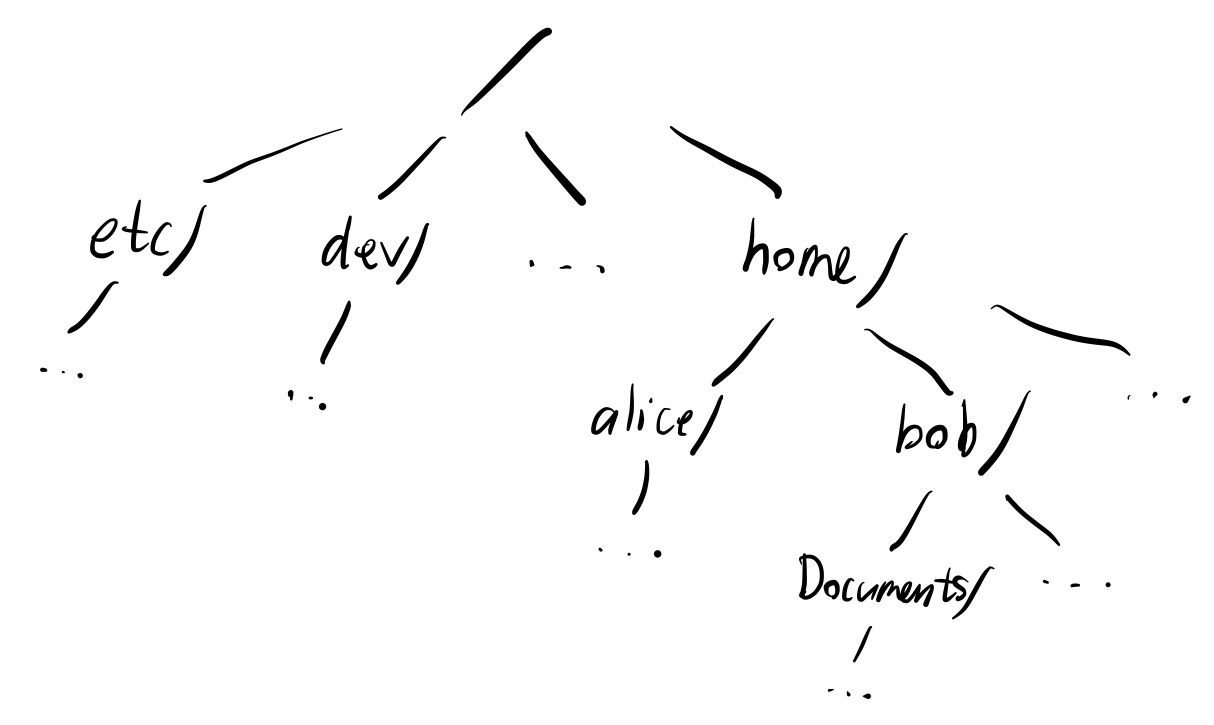
\includegraphics[scale=0.3]{3.4b.jpg}
    \item The metadata of a file contains information such as file size, file type, location, access control information, and time and date created/modified.
    \item In a hard link, a file name refers straight to an i-node. Most file metadata must be stored in the i-node and cannot be stored with the file itself, but the file name needs to be stored with each file as the different hard links can have different names.
    \item In a soft link, a file name refers to another file, not straight to an i-node. File metadata is stored with the original i-node, except once again the file name.
\end{enumerate}

\subsection*{3.6}
\begin{enumerate}[(a)]
    \item Blocking IO is the simplest to implement and use. The process is suspended until the blocked IO returns. Non-blocking IO returns almost immediately, and returns whatever is available when requested. Asynchronous IO executes while the process runs. It is the most complex to implement but is very useful as the process can continue doing other tasks while waiting for IO.
    \item \begin{itemize}
        \item To cope with impedance mismatches, buffering can be used, where the OS buffers data in memory when it arrives.
        \item Context switching can be minimised to avoid wasted computing and time.
        \item Polling or large transfers can be used to minimise the number of interrupts.
        \item A DMA device can be used to reduce the number of interrupts.
    \end{itemize}
\end{enumerate}

\section*{Tripos Question 2009/II/3a}

\begin{enumerate}[(i)]
    \item \begin{itemize}
        \item After context switching, if the data required is stored in a different place in physical memory that won't cause any problems as it will still have the same virtual memory address.
        \item The programmer cannot know which address the process will occupy at runtime, so referring to logical addresses and translating them to physical addresses at runtime is necessary.
        \item A process can't easily access data it is not allowed to access as it can't choose to just access anywhere in physical memory, and only accesses what is in its own virtual memory space, corresponding to parts of main memory it can access.
    \end{itemize}
    \item Done above (Example sheet 2 question 6a).
    \item Done above (Example sheet 2 question 6a).
    \item 
\end{enumerate}

\section*{Tripos Question 2015/II/4}
\begin{enumerate}[(a)]
    \item A page fault occurs when a frame isn't in memory. If this is due to an invalid reference, the process is killed. If it has just not been read into memory yet it is read into memory.
    \item A segment fault occurs when a process tries to access a memory address it does not have sufficient access to. When this happens on a stack segment, it means the process is trying to read or write data in an address that belongs to a different process, so a response would be to kill the process.
    \item 
    \item Page thrashing occurs when there are too many frames in memory and too many processes running so processes just end up stealing frames from each other, massively decreasing performance. This can be alleviated by decreasing the level of multiprogramming, i.e. decreasing the number of processes in progress.
    \item With an interrupt, the OS just needs to work out what caused the interrupt fulfill the request if it has sufficient permissions. In the case of a page fault, there are multiple possible causes for the fault. The first is that the process simply does not have the required permissions, so the process should be killed. The second is that it does have the relevant permissions, but the frame required is not in memory, so it has to be loaded in, and then the instruction needs to be run again.
\end{enumerate}

\end{document}
